See Fig. \ref{fig:3.5.3_towns_py}.
\begin{align}
\vec{A}=\myvec{0\\0}, 
\vec{B}=\myvec{36\\15}
\end{align}
The distance d between A and B is given by
\begin{align}
 \norm{\vec{B}-\vec{A}} &= \norm{\vec{B}}
\\
&=39km
\end{align}
 The  following Python code generates Fig. \ref{fig:3.5.3_towns_py}.
%
\begin{lstlisting}
solutions/3/codes/line/towns/towns.py
\end{lstlisting}
\begin{figure}[!ht]
\centering
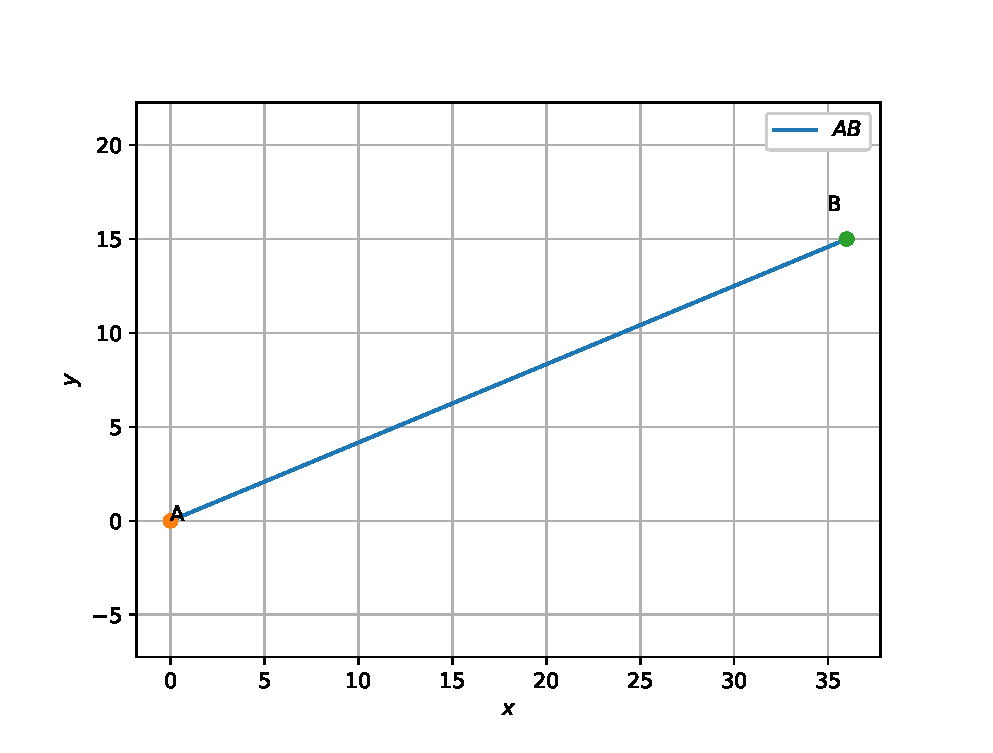
\includegraphics[width=\columnwidth]{./solutions/3/codes/line/towns/pyfigs/towns.eps}
\caption{Position of Towns A and B}
\label{fig:3.5.3_towns_py}
\end{figure}
